\documentclass[10pt,a4paper,twoside,titlepage]{article}
\usepackage[utf8]{inputenc}
\usepackage[english]{babel}
\usepackage[T1]{fontenc}
\usepackage[a4paper,top=2.54cm,bottom=2.54cm,left=3.17cm,right=3.17cm]{geometry}
\usepackage{graphicx}
\usepackage{indentfirst}
\usepackage{numprint}
\graphicspath{{images/}}
% to include more paths: \graphicspath{{images_1/},{images_2/}}
\DeclareGraphicsExtensions{.png, .pdf, .jpeg, .EPS} % image extensions
\usepackage[plainpages=false,pdfauthor={Piero Dalle Pezze},pdftitle={Manual for Rainbow - A Simulator of Computer Processes and Resources},pdftex]{hyperref}
\hypersetup{colorlinks=true,linkcolor=blue} % set colorlinks to true to enable colors (to remove for printing purposes)
\usepackage{url}
\usepackage[all]{hypcap}
\usepackage{color}
\usepackage{setspace}
\usepackage[footnotesize]{caption}








\begin{document}


%opening    
\begin{titlepage}
  \title{Manual for\\ Rainbow: A simulator of computer processes and resources}
  \author{Piero Dalle Pezze}    
\end{titlepage}

\maketitle


\newpage
The Rainbow Documentation Team - Copyright © 2006-2016 \\
\textbf{Legal notes:} Permission is granted to copy, distribute and/or modify this document under the terms of the GNU Free Documentation License, Version 1.3 or any later version published by the Free Software Foundation; with no Invariant Sections, no Front-Cover Texts, and no Back-Cover Texts. A copy of the license is included in the section entitled "GNU Free Documentation License".
\newpage



\tableofcontents
\listoffigures
\listoftables


\newpage



\section{Introduction}
\label{sec:introduction}
This is an open source software designed to support graduate and senior students, teachers and people, interested to understand the dynamic of how processes execute in a multitasking computer by simulating their behaviour. So, it offers the possibility to see and deepen in a graphic and textual point of view lots of theoretical and practical results. 



\section{How to report a bug or a communication}
\label{sec:how_to_report_a_bug_or_a_communication}
You can notify any failure or error by sending a mail to the following address: piero.dallepezze@gmail.com. It is important that you give a careful description of the problem signaled, reporting the scenario and the conditions (data input) by which you suppose the software does not work correctly.



\section{General description}
\label{sec:general_description}
This software provides a graphic and textual simulation of processes and resources in a multitasking computer. Its aim is to study how processes execute using different scheduling and accessing to resources policies. The main GUI of Rainbow is shown in Figure \ref{fig:main_window}. 
\begin{figure}[tb]
	\begin{center}
		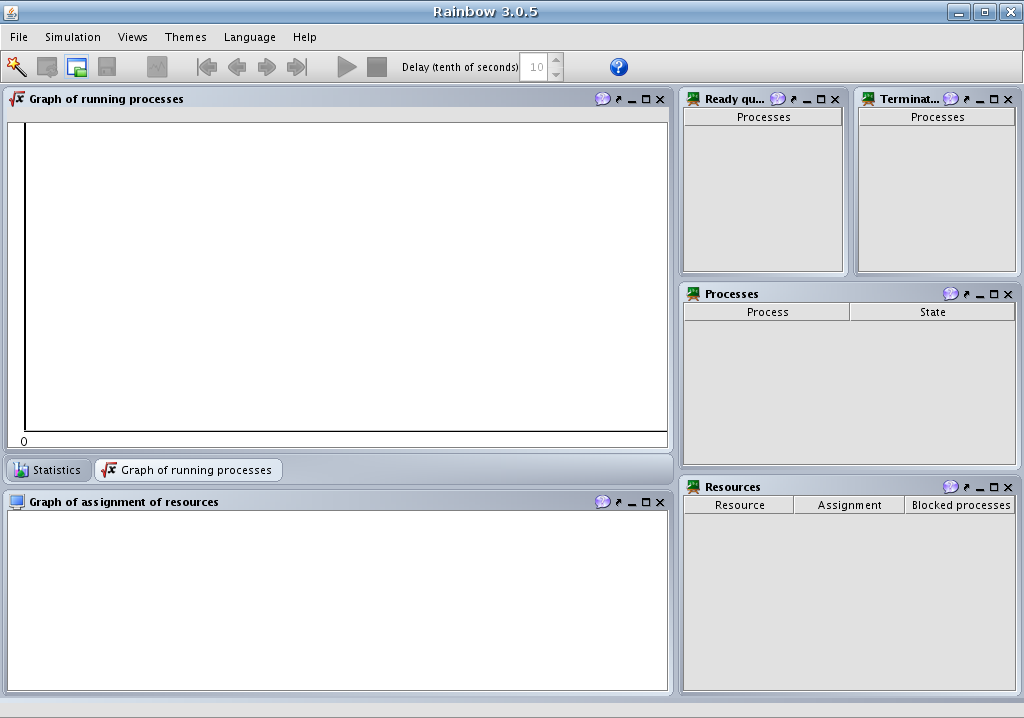
\includegraphics[scale=0.4]{main_window}
		\caption[The main frame of Rainbow]{The main frame of Rainbow.}
		\label{fig:main_window}
	\end{center}
\end{figure}
The user can see: \\
\begin{itemize}
 \item for each process, its actual state;
 \item for each resource, the processes blocked and which are using it;
 \item a graph of resource allocation;
 \item a graph representing the scheduling function;
 \item the list of ready processes;
 \item the list of terminated processes;
 \item the simulation statistics.
\end{itemize}



\section{Minimal requirements}
\label{sec:minimal_requirements}
This software is written in Java programming language. So, it works correctly in every operating system with a Java Virtual Machine installed. In general, these are the minimum requirements:
\begin{itemize}
 \item \textbf{Software requirements}: Java v1.7, Infonode GUI libraries 1.6.1 (included, GPL license), JGoodies GUI libraries 2.2.2 (included, BSD license), Swing-layout GUI libraries 1.0.3 (included, LGPL license). Use `mvn package` to retrieve these dependencies using Maven.
 \item \textbf{Hardware requirements}: Processor 800 MHz, 128 MB RAM. 
\end{itemize}



\section{Functional description}
\label{sec:functional_description}

\subsection{Rainbow configuration}
\label{subsec:rainbow_configuration}
The file config.xml, inside the folder config/, contains the configurations of the software Rainbow. By editing this file, the user can change default values. 
The default configuration of Rainbow is shown in Table \ref{tab:default_config}.


\begin{center}
\begin{table}[tb]
    \begin{tabular}{ | l | l | l |}
    \hline
    \textbf{Entry} & \textbf{Default value} & \textbf{Limit} \\ \hline
    Maximum number of processes & 100 & 100 \\ \hline
    Maximum number of resources & 100 & 100 \\ \hline
    Maximum number of accesses & 500 & 500 \\ \hline
    Maximum activation time & 100 & 100 \\ \hline
    Maximum execution time & 100 & 100 \\ \hline
    Minimum priority & -50 & -200 \\ \hline        
    Maximum priority & 50 & 200 \\ \hline
    Minimum ceiling priority & 0 & 0 \\ \hline        
    Maximum ceiling priority & 99 & 99 \\ \hline    
    Maximum multiplicity & 99 & 99 \\ \hline
    Maximum quantum & 99 & 99 \\ \hline
    Number of levels in Multilevel Feedback policies & 10 & 10 \\ \hline        
    Language & English & - \\ \hline
    Theme & Shaped Gradient Theme & - \\ \hline
    Look And Feel & JGoodies & - \\
    \hline
    \end{tabular}
    \caption[Default configuration of Rainbow]{Default configuration of Rainbow.}    
    \label{tab:default_config}    
\end{table}    
\end{center}




\subsection{Configuration of a simulation}
\label{subsec:configuration_of_a_simulation}
Before starting a simulation, the user must create a configuration. 
Depending on whether an user knows the set of processes that the system will execute a priori, Rainbow offers two types of configuration: random or manually configured. A random configuration is a configuration in which the processes, resources and accesses of processes to resources are randomised (within the limits of Rainbow). In a manual configuration, the user creates the sets of processes, resources and accesses entirely. The latter is achieved using the standard panel of Rainbow, called Data Input. This panel is also invokable when an open configuration is to be changed. After the user has clicked on the Accept button, the simulation is ready.
The panel used to configure a simulation is made of four tabs:

\subsubsection{Processes}
\label{subsubsec:Processes}
By using a form module, the user can specify all data about processes. Moreover tool-tips shows all input limits. Each process is characterized by a name, an activation time, an execution time and an initial priority. See Figure \ref{fig:config_processes}.
\begin{figure}[tb]
	\begin{center}
		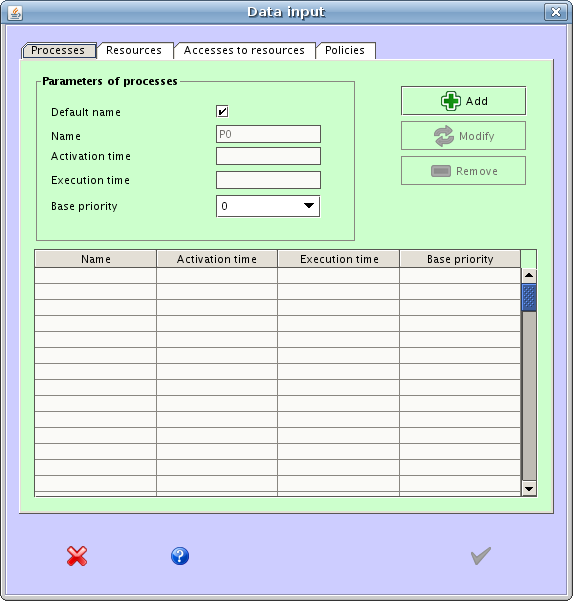
\includegraphics[scale=0.6]{config_processes}
		\caption[Configuration of the processes]{Configuration of the processes.}
		\label{fig:config_processes}
	\end{center}
\end{figure}


\subsubsection{Resources}
\label{subsubsec:resources}
By using a form module, the user can specify all data about resources. Moreover tool-tips shows all input limits. Each resource is characterized by a name and a multiplicity. A resource can be preemptive or not preemptive. In the second case, the user can also specify the ceiling priority if ICPP flag is selected. See Figure \ref{fig:config_resources}.
\begin{figure}[tb]
	\begin{center}
		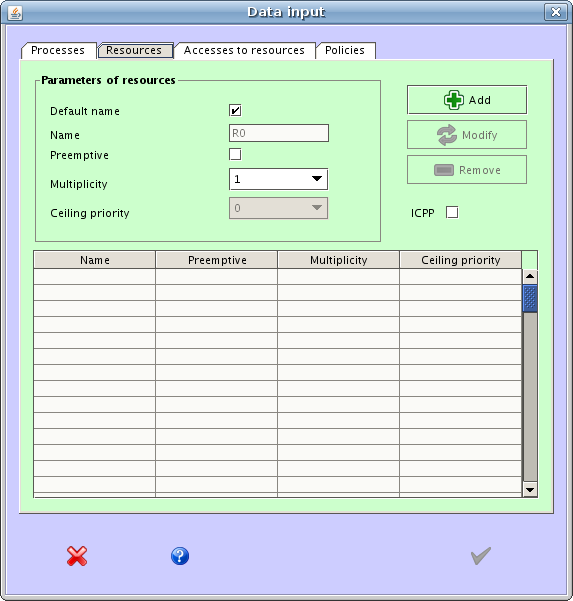
\includegraphics[scale=0.6]{config_resources}
		\caption[Configuration of the resources]{Configuration of the resources}
		\label{fig:config_resources}
	\end{center}
\end{figure}


\subsubsection{Accesses to resources}
\label{subsubsec:accesses_to_resources}
By using a form module, the user can specify all data about accesses to resources by processes. Moreover tool-tips shows all input limits. Each access concern a process and a resource created. The user can specify the request time and the time of the access. See Figure \ref{fig:config_accesses}.
\begin{figure}[tb]
	\begin{center}
		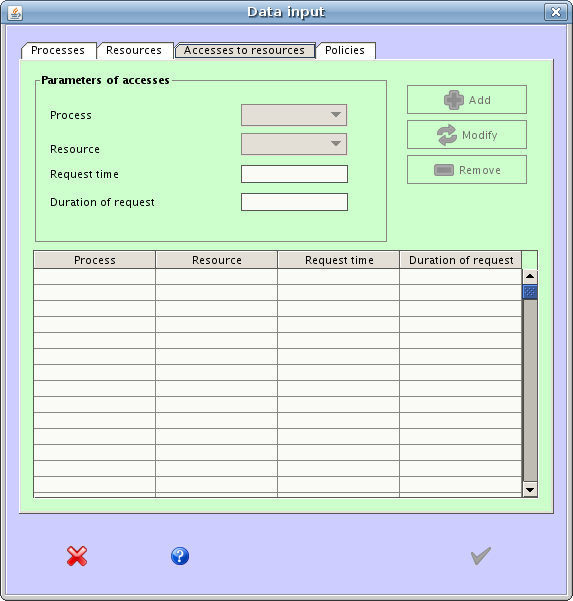
\includegraphics[scale=0.6]{config_accesses}
		\caption[Configuration of the accesses]{Configuration of the accesses.}
		\label{fig:config_accesses}
	\end{center}
\end{figure}


\subsubsection{Policies}
\label{subsubsec:policies}
By using a form module, the user can specify all data about scheduling and assignment policies. In particular the user can choose the scheduling and assignment policies to use. If the selected scheduling policy is a time sharing one, the quantum value is also configurable. See Figure \ref{fig:config_policies}.
\begin{figure}[tb]
	\begin{center}
		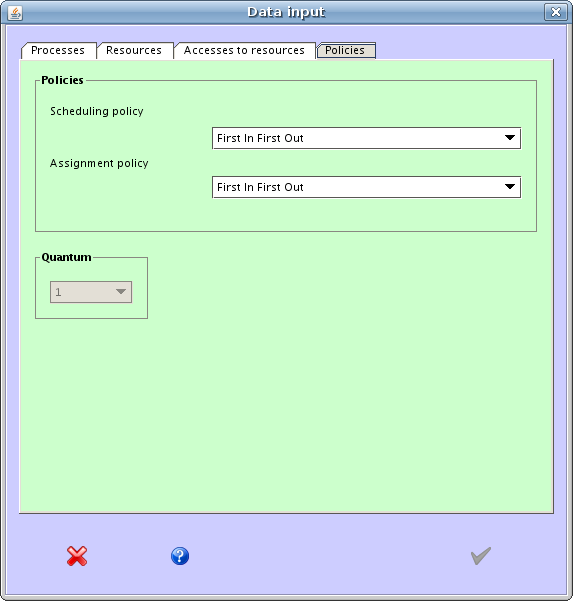
\includegraphics[scale=0.6]{config_policies}
		\caption[Configuration of the policies]{Configuration of the policies.}
		\label{fig:config_policies}
	\end{center}
\end{figure}



\subsection{Simulation}
\label{subsec:simulation}
An user can start the simulation and advance it manually. The graphical user interface, is subdivided in several views which allow to analysis the most relevant details. See Figures \ref{fig:rainbow_simulation} and \ref{fig:rainbow_statistics}. The views in Rainbow concern: 
\begin{itemize}
 \item The graph of running processes 
 \item The graph of the current allocation of resources 
 \item The ready queue
 \item The list of processes terminated 
 \item The states of processes 
 \item The resources and lists of blocked processes 
 \item The statistics 
\end{itemize}

\begin{figure}[tb]
	\begin{center}
		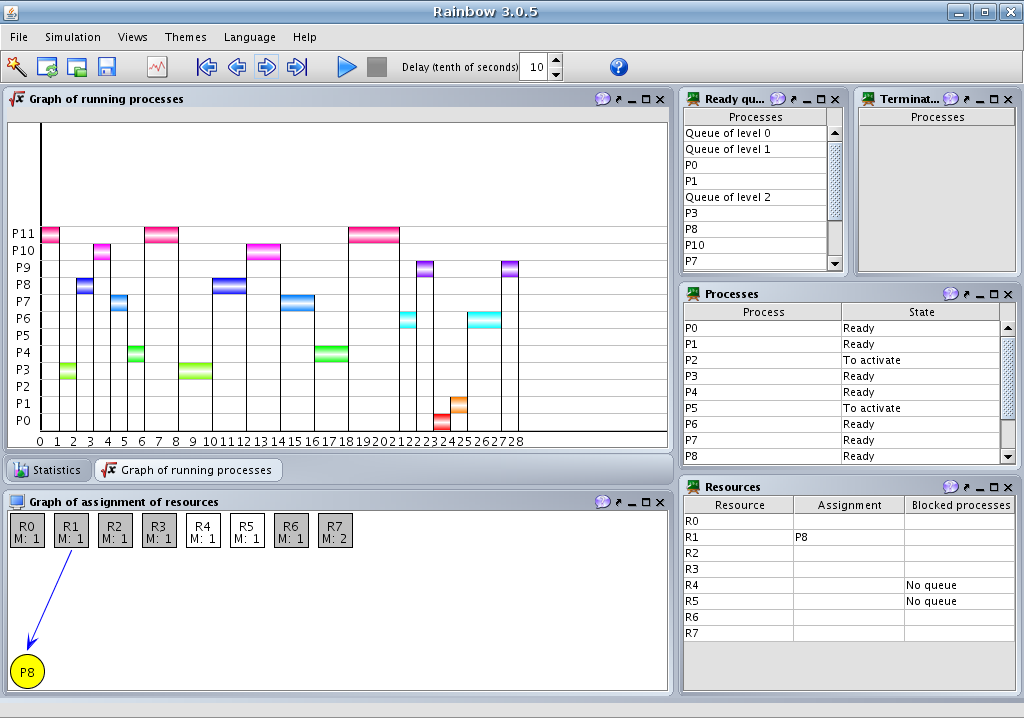
\includegraphics[scale=0.4]{rainbow_simulation}
		\caption[An example of simulation]{An example of simulation using Multilevel Feedback scheduling policy and FIFO assignment policy.}
		\label{fig:rainbow_simulation}
	\end{center}
\end{figure}
\begin{figure}[tb]
	\begin{center}
		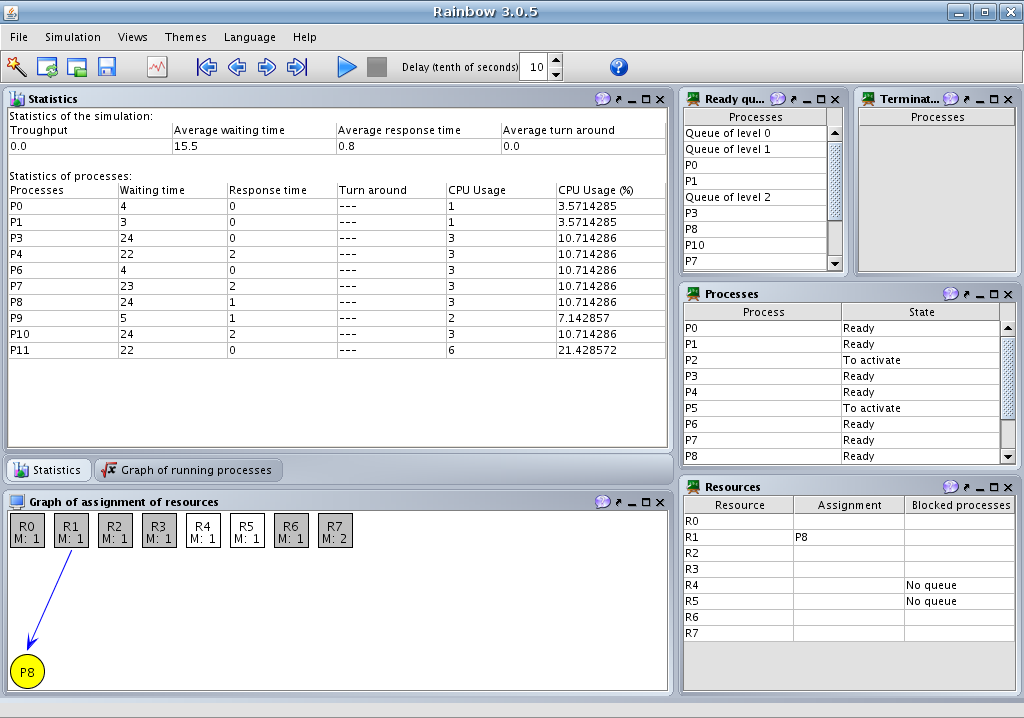
\includegraphics[scale=0.4]{rainbow_statistics}
		\caption[An example of statistics view]{Statistics for the previous example using Multilevel Feedback scheduling policy and FIFO assignment policy.}
		\label{fig:rainbow_statistics}
	\end{center}
\end{figure}



\subsubsection{The graph of running processes}
\label{subsubsec:The graph of running processes}
This window illustrates the scheduling function. So it shows the order of execution of processes. The time of context switch is null. If the selected process cannot execute because it must to access to a non-free resource, then it becomes blocked and the CPU runs nothing for an unit of time.

\subsubsection{The graph of the current allocation of resources}
\label{subsubsec:The graph of the current allocation of resources}
Here it is shows the current allocation of resources to processes. Processes are represented with a colored circle with their name reported inside. Instead, resources are pictured with a square with their name and multiplicity reported inside. The white color notifies that it is preemptive, the gray one if the resource is non-preemptive. The relation between a process and a resource is identified by an arrow. If a process asks a non-free resource, an arrow is directed from the process to the resource. If a process detains a resource, an arrow is directed from the resource to the process.

\subsubsection{The ready queue}
\label{subsubsec:The ready queue}
In this window, the ready queue is represented. Processes are sorted by the scheduling policy adopted. In general, the first process in the queue is the next to execute. If the user chooses one of the multilevel feedback policies family, then the indexed queues are printed (see MF). if the user chooses one of the priority policies family, then for each priority a queue is printed (see HPF).

\subsubsection{The list of processes terminated}
\label{subsubsec:The list of processes terminated}
In this window, all processes terminated are reported in temporal order of termination. The first process terminated is the highest in the list.

\subsubsection{The states of processes}
\label{subsubsec:The states of processes}
In this window, all processes are listed with their current state (running, ready, terminated, blocked, to activate).

\subsubsection{The resources and lists of blocked processes}
\label{subsubsec:The resources and lists of blocked processes}
This window reports all resources with the list of processes to whom it is allocated and the queue of processes blocked, sorted by the assignment policy (if the resource is non-preemptive).

\subsubsection{Statistics}
\label{subsubsec:statistics} 
This window shows the main statistics of the simulation and processes until the current time. It is possible to see the statistics by clicking the button "Show statistics". The statistics are divided in two parts. The first one regards the simulation and includes the throughput, the average waiting time, the average response time and the average turn around time. The second one concerns processes involved in the simulation and shows for each of them, its waiting time, response time, turn around time, CPU usage and the CPU usage percentage.




\subsection{Multi language}
\label{subsec:Multi language}
From the third version, this software supports multi language.
Available languages are: English, Italian, German, French, Spanish, Portuguese, Dutch, Danish, Swedish, Norwegian, Finnish, Russian, Ukrainian, Polish, Greek, Japanese, Korean, Chinese (Simple and Traditional), Arabic, Indonesian, Hungarian, Persian, and Esperanto.


\subsection{Menu bar}
\label{subsec:Menu bar}
The complete list of menus is the following:
\begin{itemize}
 \item File
 \item New (it creates a new configuration) 
 \item Open (it opens the current configuration) 
 \item Save (it saves the current configuration) 
 \item Modify (it modifies the current configuration) 
 \item Export (html) (it exports the current configuration in html format)
 \item Import (fcs) (it imports the current configuration in fcs format) (retro-compatibility)
 \item Exit (it exits from Rainbow) 
\end{itemize}

\subsubsection{Simulation}
\label{subsubsec:Simulation} 
It contains all buttons to surf the simulation. These are present also in the tool bar. There is a button to visualize the current configuration inserted.

\subsubsection{Views}
\label{subsubsec:Views} 
The default layout button allows to return to the standard layout of Rainbow. The maximum layout button allows to maximize views adopting the tab visualization. So it is possible to see the simulation of configurations with a lots of data in a comfortable way. All other buttons turn on or off the respective views.

\subsubsection{Themes}
\label{subsubsec:Themes} 
A list of themes to change the look and feel of Rainbow.

\subsubsection{Language}
\label{subsubsec:Language} 
The list of the available languages with their flags. When one is selected, Rainbow is automatically translated into that language. The next time that Rainbow will be executed, the selected language in the previous session will be restored.

\subsubsection{Help}
\label{subsubsec:Help} 
Used to recall the help and the about functionalities. In every moment, the user can call the main or context sensitive help, by clicking in the help menu, or in the question mark of a view.





\section{Appendix}
\label{sec:Appendix}


\subsection{Glossary}
\label{subsec:Glossary}

\begin{description}
 \item [Attribution] It shows processes to whom the resource is attributed.
 \item [Deadlock] A set of processes is in a deadlock state if every process waits an event that only another process in the same set can throw. There are four conditions to rise a deadlock: 1. Mutual exclusion: every resource can be accessed by only a process; 2. Hold and wait: processes, that obtain resources, can ask other ones; 3. No preemption: A resource assigned to a process cannot be subtracted to it until the voluntary release of the process; 4. Circular waiting: there is a circular chains of requests among processes to resources. 
 \item [Multiplicity] It is the maximum number of processes that a resource can be attributed in the same time. A resource with multiplicity 1 and no preemptive, is said to be accessed in mutual exclusion way.
 \item [Assignment policy] An assignment policy sorts the queue of blocked processes. It determines how blocked processes wake up when the resource waited becomes available.
 \item [Scheduling policy] A scheduling policy sorts the ready queue. It determines how ready processes are dispatched to the CPU.
 \item [Process] A process is a program in execution. Inside an operating system, a process control block (PCB) manages current values of program counter registers and other variables. A PCB is an entry of the process table, which is manages by the scheduler. In this application processes are abstraction of real ones.
 \item [Resource] A resource is everything can be accessed and used. P.E. a file, a device, a function etc. A resource can be preemptive or not preemptive.
 \item [No preemptive resource] It is a resource that cannot be subtracted to a process that is using it.
 \item [Preemptive resource] It is a resource that can be subtracted to a process that is using it.
 \item [Simulation] It is the temporal evolution of the management of processes.
 \item [Batch system] A batch system is characterized by a determined sorting, no preemptive, long execution jobs. This approach reduces context switch among processes, improving performances.
 \item [Interactive system] An interactive system is characterized by a great variety of activities. The preemption is needed.
 \item [Real time system] A real time system is characterized by short execution processes, often with deadline. Sometimes the preemption is not needed. Real time systems are divided into soft real time, which are systems where the deadline is important but not critical, and hard real time, where the respect of the execution before deadline is crucial.
 \item [State of a process] The states of a process are: to activate, ready, running, blocked, terminated. A process is said: ``about to be active'' when it is declared but not activated; ``ready'' when it is ready to execute (see scheduling policy for details); ``running'' when it is using the CPU to execute; ``blocked'' when it is waiting a non preemptive resource which is unavailable because allocated to another (others) processes (see multiplicity). In this case, a request of access of the process is queued on the wanted resource (see assignment resource); and ``terminated'' when it has completed its execution.
 \item [Response time] It is the time perceived by the end user is the interval between the instant at which an operator at a terminal enters a request for a response from a computer and the instant at which the first character of the response is received at a terminal.
 \item [Turn around time] It is the time between the placement of an order and its delivery.
 \item [Throughput] It is the number of job per hour that the system is able to complete.
 \item [Time slice] The period of time for which a process is allowed to run in a preemptive multitasking system is generally called the "time slice". The scheduler is run once every time slice to choose the next process to run. If the time slice is too short then the scheduler will consume too much processing time but if it is too long then processes may not be able to respond to external events quickly enough.
 \item [Waiting time] It is the time when the process is waiting for execution.
\end{description}


\subsection{Scheduling policies}
\label{subsec:Scheduling policies}
In this paragraph, all available scheduling policies are described: 
\begin{description}
 \item [FIFO: (First In First Out)] This is a policy for batch system. It holds the ready queue sorted by FIFO. So the first process added to the queue is the first to be extracted by the dispatcher. 
 \item [SJF: (Shortest Job First)] This is a policy for batch system. It holds the ready queue sorted by execution time increasing. So it will extract always the process with minimum execution time. 
 \item [SRTF: (Shortest Remain Time First)] This is a policy for batch system. It is a variant of SJF policy because it apply the preemption of the running process when a process with a minor execution time is inserted in the queue. 
 \item [Round Robin:] This is a policy for interactive system. It holds the ready queue sorted by FIFO, but executes the running process per a quantum of time. When the quantum expires, the running process is put to the tail of the queue. The quantum is also called time slice. 
 \item [Round Robin with Priority:] This is a policy for interactive system. It is a variant of the classic round robin policy. On details, it holds the ready queue sorted by priority decreasing. So it will extract always the process with the highest priority. 
 \item [Preemptive on Priority Round Robin:] This is a policy for interactive system. It is a variant of the round robin with priority policy. On details, it applies the preemption of the running process when a process with higher priority is inserted in the queue. 
 \item [HPF: (Highest Priority First)] This is a policy for interactive system. It holds the ready queue sorted by priority decreasing. So it will extract always the process with the highest priority. 
 \item [Preemptive HPF: (Preemptive Highest Priority First)] This is a policy for interactive system. It is a variant of the HPF policy. It applies the preemption of the running process when a process with higher priority is inserted in the queue. 
 \item [HRRN: (Highest Response Ratio Next)] This is a policy for interactive system. The response ratio of a process is so defined: response\_ratio = (expected\_execution\_time + waiting\_time) / expected\_execution\_time . It will extract always the process with the highest response ratio. 
 \item [MF: (Multilevel Feedback)] This is a policy for interactive system. The ready queue is made of several queues sorted by FIFO policy. An activated process is inserted on the tail of the queue Q0. As Round Robin, it executes the running process, which was before ready in the queue Qi, only for a quantum of time. Then the process is inserted in a queue Q(i+1). It always extracts, if exists, the process in the queue of lower level. 
 \item [Preemptive MF: (Preemptive Multilevel Feedback)] This is a policy for interactive system. It is a variant of the classic Multilevel Feedback policy. It applies the preemption of the running process when a new process is inserted in a queue of lower level than the level of the queue of the running process. 
 \item [MFDQ: (Multilevel Feedback with Dynamic Quantum)] This is a policy for interactive system. It is a variant of the classic Multilevel Feedback policy. The quantum value depends on the level of the queue. On details: queue of level 0 : dynamic\_time\_slice = time\_slice; queue of level i-th: dynamic\_time\_slice(i) = 2 * dynamic\_time\_slice(i-1). So a process executes for a quantum of time as longer as the level of queue is higher. 
 \item [Preemptive MFDQ: (Preemptive Multilevel Feedback with Dynamic Quantum)] This is a policy for interactive system. This is a variant of the Multilevel Feedback with Dynamic Quantum policy. It applies the preemption of the running process when a new process is inserted in a queue of lower level than the level of the queue of the running process. 
 \item [Linux:] This is a policy for interactive system. It is the Linux scheduling policy. See references for details. (Not supported yet!)
 \item [UNIX:] This is a policy for interactive system. It is the UNIX scheduling policy. See references for details. (Not supported yet!)
\end{description}


\subsection{Assignment policies}
\label{subsec:Assignment policies}
In this paragraph, all available assignment policies are described:
\begin{description}
 \item[First In First Out:] This policy holds the queue of requests of processes to a resource sorted by FIFO. So the first process blocked in the queue is the first signaled in the queue when the non-preemptive resource will become available. 
 \item[Highest Priority First:] This policy holds the queue of requests of processes to a resource sorted by HPF. So the first process signaled when the non-preemptive resource will become available is the process with the highest dynamic priority in the queue. 
 \item[Random:] This policy holds the queue of requests of processes to a resource sorted by FIFO. However, the process signaled when the non-preemptive resource will become available is chosen in a random way. This policy simulates the behavior of the notify() method in Java. (By assuming in this context, processes instead of threads).
\end{description}


\clearpage
\section*{References}
\label{sec:References}
\begin{itemize}
 \item Modern Operating System by Andrew S. Tanenbaum 
 \item Operating System Concepts by Silberschatz, Galvin, Gagne 
 \item Concurrency in Ada by Burns, Wellings 
 \item Thinking in Java by Bruce Eckel 
 \item Software Engineering by Ian Sommerville 
 \item SWEBOK - Guide to the Software Engineering Body of Knowledge by IEEE 
 \item GNU
 \item Wikipedia 
\end{itemize}



\end{document}
